% !TeX spellcheck = en_US
\addsection{Round Structure}{\spells/forgetfulness.png}

\begin{multicols*}{2}

The game is structured into Rounds, during which each player will take their own Turn in a clockwise order starting with the starting player.
During their Turns, players will move their \hyperlink{Heroes}{Heroes} on the Game Map, construct new Buildings in their \hyperlink{Town}{Town} and Recruit \hyperlink{Units}{Units} in an attempt to fulfill the Scenario's victory condition.\par
Perform the following steps \textbf{at the start of every Round} except the first one:
\begin{itemize}
  \item Flip any previously used Build, Population and/or Spell Book Tokens back to their active side.
  \item Flip any previously used Movement Point (MP) Tokens back to their active, green side.
  \item Regain uses for Expert Effects \includesvg[height=10px]{\svgs/expert.svg}.
\end{itemize}
Then, depending on the current Round number, players either gain Resources or resolve an Astrologers Proclaim Card:
\begin{itemize}
  \item Odd-numbered Rounds are \textbf{Resource Rounds}.
    All players gain income from the \hyperlink{Mines}{Buildings, Settlements, and Mines} they control.
    Skip this step during the first Round.
  \item Even-numbered Rounds are \textbf{Astrologers' Rounds}.
    Draw an Astrologers Proclaim Card\index{Astrologers Proclaim Card} and resolve its effects.
  \item If the Scenario has timed Events marked on the Round Tracker that have now been reached, resolve them.
\end{itemize}
After the start of the Round, players take Turns in a clockwise order as described in the next section.
After all players have played their Turn, move the Black Cube on the Round Tracker one space forward and perform the start of Round again.
Keep playing new Rounds until any of the Scenario's ending conditions have been met.

\vspace*{\fill}

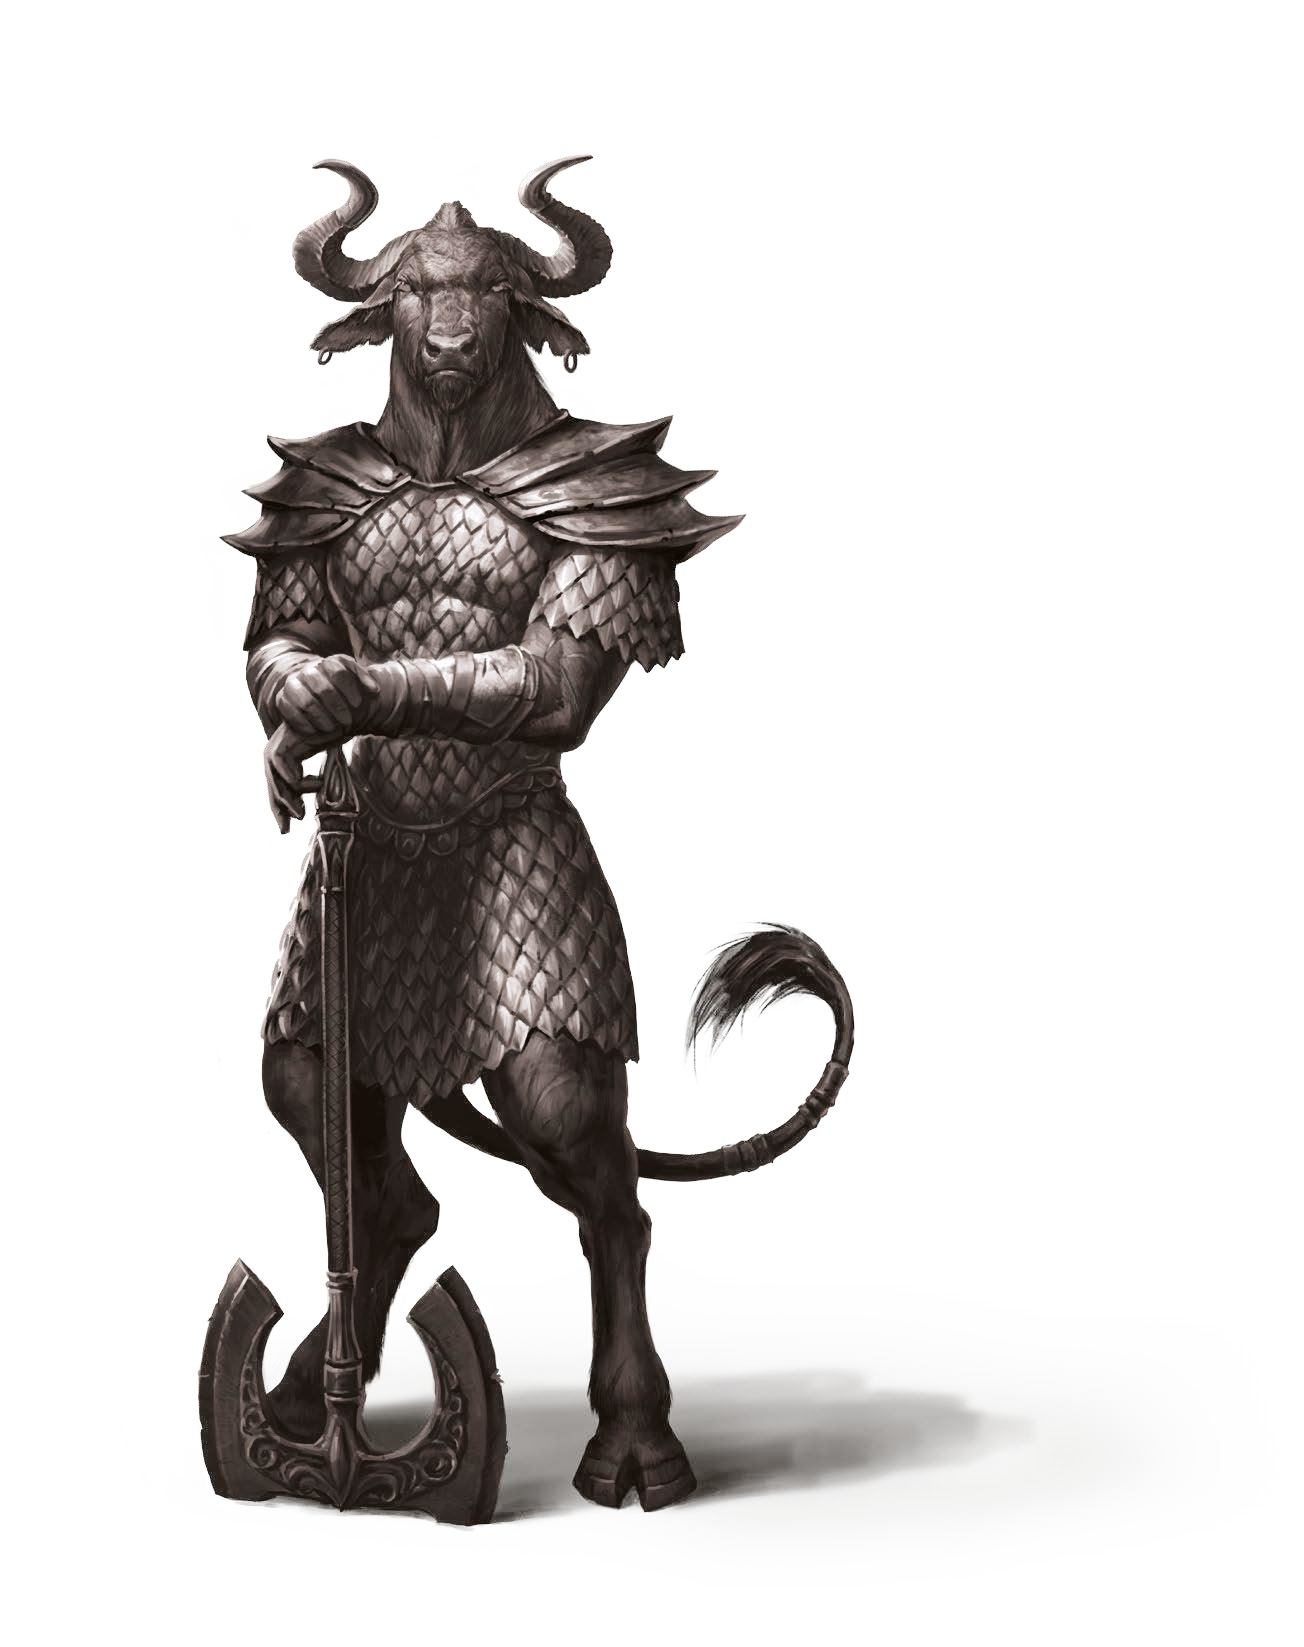
\includegraphics[width=1.8\linewidth]{\art/minotaur.png}

\end{multicols*}
